\chapter{Relazioni di Laboratorio}
In questo capitolo, illustreremo la metodica per realizzare una relazione di laboratorio di fisica. L'esempio svolto sarà abbastanza completo ma si tenga conto del fatto che, a seconda degli argomenti e del tempo a disposizione,  una relazione reale potrebbe essere diversa per varie ragioni (non sempre si realizzano grafici o si calcolano gli errori come abbiamo fatto). Nel caso trattato, abbiamo usato una tecnica (l'uso della linea di tendenza o di \textit{bestfit}) molto efficace quando si ha la possibilità di misurare la variazione di due grandezze correlate (si può usare a tal proposito il foglio di calcolo). Alcune misure però, specialmente le prime che svolgeremo, richiedono solo misure dirette e lo scopo della relazione sarà la misura di una o più grandezze e la loro  scrittura corretta (quella del tipo $x=\left( \overline{x} \pm \Delta x\right)$ per intenderci).
\section{Titolo e Scopo dell'Esperienza}
Il titolo deve essere chiaro e conciso. Lo scopo dell'esperienza deve spiegare brevemente l'obiettivo dell'esperimento.

\section{Materiali e Strumenti}
Elencare tutti i materiali e gli strumenti utilizzati, specificando la sensibilità e la portata degli strumenti di misura. Includere un'immagine dell'apparato sperimentale.

\section{Raccolta Dati}
Presentare i dati raccolti in forma tabulare, includendo gli errori nelle misure dirette.

\section{Cenni Teorici}
Esporre brevemente la teoria relativa all'esperimento, includendo le formule rilevanti.

\section{Elaborazione Dati}
Descrivere il processo di elaborazione dei dati raccolti.

\section{Calcolo degli Errori nelle Misure Indirette}
Spiegare come si propagano gli errori nelle misure indirette.

\section{Grafico Sperimentale}
Presentare i dati in forma grafica, includendo le barre di errore.

\section{Conclusioni}
Discutere i risultati ottenuti, confrontandoli con le previsioni teoriche.

\newpage

\section{Esempio: Studio del Moto}

\subsection{Titolo e Scopo dell'Esperienza}
\textbf{Titolo:} Studio del Moto Uniformemente Accelerato\\
\textbf{Scopo:} Verificare sperimentalmente le leggi del moto uniformemente accelerato.

\subsection{Materiali e Strumenti}
\begin{itemize}
    \item Piano inclinato (base \SI{2000}{\milli\metre}) e inclinato di \SI{30}{\degree}.
    \item Sfera metallica.
    \item Cronometro digitale (sensibilità: \SI{0,01}{\second}, portata: \SI{999,99}{\second}).
    \item Metro a nastro (sensibilità: \SI{1}{\milli\metre}, portata: \SI{3000}{\milli\metre}).
    \item Goniometro (sensibilità: \SI{1}{\degree}, portata: \SI{180}{\degree}).
\end{itemize}

\begin{figure}[!htbp] 
    \centering
    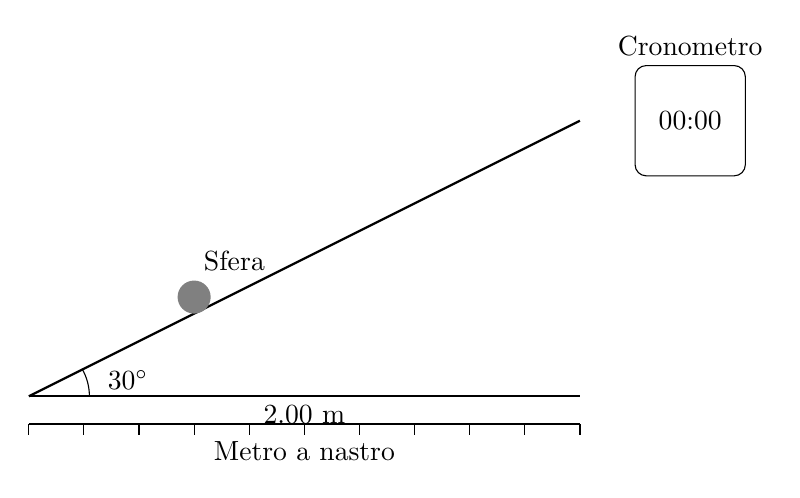
\begin{tikzpicture}[scale=0.7]
        % Piano inclinato
        \draw[thick] (0,0) -- (10,5);
        \draw[thick] (0,0) -- (10,0);
        
        % Sfera
        \fill[gray] (3,1.8) circle (0.3);
        
        % Cronometro
        \draw[rounded corners] (11,4) rectangle (13,6);
        \node at (12,5) {00:00};
        
        % Metro a nastro
        \draw[thick] (0,-0.5) -- (10,-0.5);
        \foreach \x in {0,1,...,10}
            \draw (\x,-0.7) -- (\x,-0.5);
        \node at (5,-1) {Metro a nastro};
        
        % Goniometro
        \draw (1.1,0) arc (0:30:1);
        \node at (1.8,0.3) {$30^\circ$};
        
        % Etichette
        \node[below] at (5,0) {2.00 m};
        \node[above right] at (3,2.1) {Sfera};
        \node[above] at (12,6) {Cronometro};
    \end{tikzpicture}
    \caption{Apparato sperimentale per lo studio del moto uniformemente accelerato.}
    \label{fig:apparato}
\end{figure}

\subsection{Raccolta Dati}
Abbiamo misurato il tempo impiegato dalla sfera per percorrere diverse distanze lungo il piano inclinato, inclinato di \SI{30}{\degree} rispetto all'orizzontale.

\begin{table}[!htbp] 
    \centering
    \begin{tabular}{@{}ccc@{}}
        \toprule
        Distanza (\si{\metre}) & Tempo (\si{\second}) & Errore sul tempo (\si{\second}) \\
        \midrule
        0,200 & 0,29 & 0,01 \\
        0,400 & 0,41 & 0,01 \\
        0,600 & 0,50 & 0,01 \\
        0,800 & 0,58 & 0,01 \\
        1,000 & 0,65 & 0,01 \\
        \bottomrule
    \end{tabular}
    \caption{Dati sperimentali}
    \label{tab:datitab}
\end{table}

\subsection{Cenni Teorici}
Nel moto uniformemente accelerato, la posizione $s$ in funzione del tempo $t$ è data da:

\begin{equation}
    s = \frac{1}{2}at^2
\end{equation}

dove $a$ è l'accelerazione. Nel nostro caso, l'accelerazione lungo il piano inclinato è data da:

\begin{equation}
    a = g\sin\theta
\end{equation}

dove $g$ è l'accelerazione di gravità e $\theta$ è l'angolo di inclinazione del piano.

\subsection{Elaborazione Dati}
Per verificare la relazione $s = \frac{1}{2}at^2$, plotteremo $s$ in funzione di $t^2$.
 La pendenza della retta di best fit sarà $\frac{1}{2}a$. Prima di realizzare il grafico,
 calcoliamo anzitutto gli errori e poi metteremo i punti sul piano cartesiano. In fine calcoleremo
 l'accelerazione di gravità dalla pendenza. I dettagli per farlo sono riassunti nei paragrafi
 sull'uso del foglio di calcolo (o con la procedura manuale).

\subsection{Calcolo degli Errori nelle Misure Indirette}
L'errore su $t^2$ si propaga come:

\begin{equation}
    \Delta(t^2) =\overline{t^2} \left(2\cdot\frac{\Delta t}{\overline{t}}  \right)= 2\overline{t}\Delta t.
\end{equation}
Con questa formula, calcoliamo gli errori su $t^2$ e li mettiamo in tabella \ref{tab:tquadro}:

\begin{table}[h!]
\centering
\begin{tabular}{|c|c|}
\hline
$t^2$ (\si{\second\squared}) & $\Delta \left( t^2 \right)$ (\si{\second\squared}) \\
\hline
0,0841 & 0,006 \\
0,1681 & 0,008 \\
0,25   & 0,01   \\
0,3364 & 0,01 \\
0,4225 & 0,01  \\
\hline
\end{tabular}
\caption{Valori calcolati di $t^2$ e $\Delta t^2$}
\label{tab:tquadro}
\end{table}

\subsection{Grafico Sperimentale}

\begin{figure}[!htbp] 
    \centering
    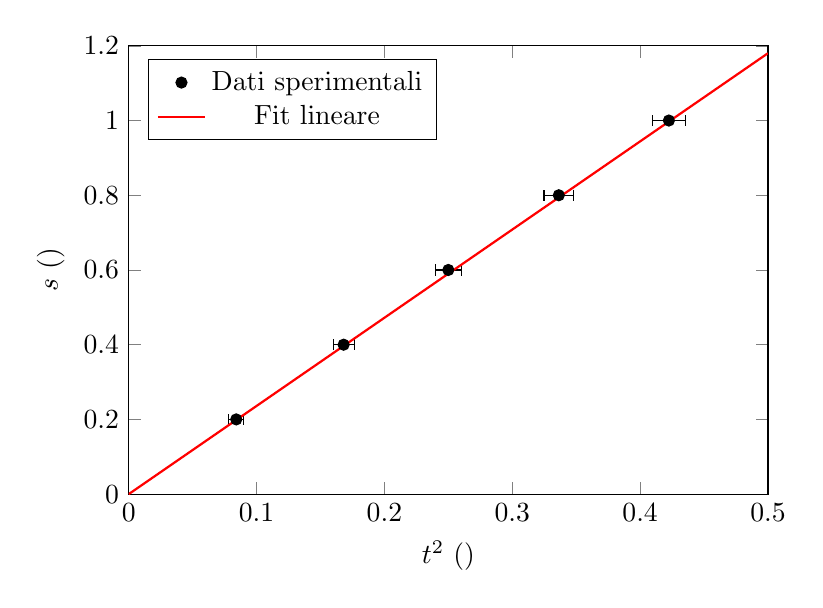
\begin{tikzpicture}
        \begin{axis}[
            width=0.8\textwidth,
            height=0.6\textwidth,
            xlabel={$t^2$ (\si{\second\squared})},
            ylabel={$s$ (\si{\metre})},
            xmin=0, xmax=0.5,
            ymin=0, ymax=1.2,
            legend pos=north west,
            ]
            \addplot[only marks,error bars/.cd,x dir=both,x explicit,y dir=both,y explicit]
            coordinates {
                (0.0841, 0.20) +- (0.0058, 0.001)
                (0.1681, 0.40) +- (0.0082, 0.001)
                (0.2500, 0.60) +- (0.0100, 0.001)
                (0.3364, 0.80) +- (0.0116, 0.001)
                (0.4225, 1.00) +- (0.0130, 0.001)
            };
            \addplot[domain=0:0.5, samples=100, smooth, thick, red] {2.3604*x};
            \legend{Dati sperimentali, Fit lineare}
        \end{axis}
    \end{tikzpicture}
    \caption{Grafico di $s$ in funzione di $t^2$.}
    \label{fig:grafico-moto}
\end{figure}
Il grafico con le barre di errore è stato ottenuto con un software perché non è possibile realizzarlo coi fogli google (non si possono inserire barre di errore personalizzate ad esempio). Ovviamente si può realizzare un ottimo grafico manuale con le tecniche esposte nei precedenti paragrafi.
\subsection{Conclusioni}
Dal fit lineare dei dati, abbiamo ottenuto una pendenza di \SI{2.3604}{\metre\per\second\squared}, che corrisponde a $\frac{1}{2}a$. La pendenza si misura sul grafico tracciando la retta a mano  oppure, se si è realizzato il grafico col foglio di calcolo, basta fargli scrivere l'equazione che sarà del tipo $y= bx +a$, dove $b$ è la pendenza. Quindi, l'accelerazione sperimentale è:

\begin{equation}
    a_{\text{exp}} = \SI{4.7208}{\metre\per\second\squared}
\end{equation}

Teoricamente, l'accelerazione dovrebbe essere:

\begin{equation}
    a_{\text{th}} = g\sin\theta = \SI{9.81}{\metre\per\second\squared} \cdot \sin(\SI{30}{\degree}) = \SI{4.905}{\metre\per\second\squared}
\end{equation}

La differenza relativa tra il valore sperimentale e quello teorico è:

\begin{equation}
    \frac{|a_{\text{exp}} - a_{\text{th}}|}{a_{\text{th}}} \cdot 100\% = \frac{|\SI{4.7208}{\metre\per\second\squared} - \SI{4.905}{\metre\per\second\squared}|}{\SI{4.905}{\metre\per\second\squared}} \cdot 100\% \approx 3.75\%
\end{equation}

Notiamo che non abbiamo potuto fare il confronto col metodo degli errori (sezione 2.4) perché non abbiamo calcolato l'errore sull'accelerazione e sul valore teorico atteso (sarebbe stato troppo complicato). Comunque, questa discrepanza del 3.75 \% tra il valore sperimentale e quello teorico è accettabile per un esperimento di laboratorio di fisica elementare. Le possibili fonti di errore includono:

\begin{itemize}
    \item Piccoli errori nella misurazione del tempo.
    \item Leggero attrito tra la sfera e il piano inclinato.
    \item Possibile imprecisione nella misurazione dell'angolo di inclinazione.
    \item Errori di parallasse nella lettura delle distanze.
\end{itemize}

Per migliorare ulteriormente l'esperimento, si potrebbe:
\begin{itemize}
    \item Utilizzare un sistema di rilevamento del tempo più preciso, come un timer fotoelettrico.
    \item Ridurre l'attrito utilizzando una superficie più liscia o una sfera con minore attrito.
    \item Ripetere le misurazioni più volte per ogni distanza per ridurre gli errori casuali.
\end{itemize}

In conclusione, l'esperimento ha confermato con buona approssimazione la relazione tra spazio e tempo nel moto uniformemente accelerato, dimostrando l'efficacia del metodo sperimentale nell'investigare le leggi della fisica.



\section{Secondo Principio della Dinamica}

\subsection{Scopo dell'Esperimento}
L'obiettivo di questo esperimento è verificare sperimentalmente il secondo principio della dinamica di Newton, utilizzando un sistema costituito da due masse collegate da una fune inestensibile che passa attraverso una carrucola. In particolare, si vuole verificare la relazione:
\begin{equation}
    \vec{F} = m\vec{a}
\end{equation}
dove $\vec{F}$ è la forza risultante applicata al sistema, $m$ è la massa del sistema e $\vec{a}$ è l'accelerazione risultante.

\subsection{Cenni Teorici}
Il sistema sperimentale consiste in:
\begin{itemize}
    \item Un carrello di massa $m_1$ che può scorrere su un piano orizzontale
    \item Una massa $m_2$ collegata al carrello tramite una fune inestensibile
    \item Una carrucola considerata ideale (massa e attrito trascurabili)
\end{itemize}

Le equazioni del moto del sistema sono:
\begin{align}
    m_2g - T &= m_2a \\
    T - f_a &= m_1a
\end{align}
dove:
\begin{itemize}
    \item $T$ è la tensione della fune
    \item $f_a$ è la forza di attrito
    \item $a$ è l'accelerazione del sistema
    \item $g$ è l'accelerazione di gravità ($g = \SI{9,81}{\meter\per\second\squared}$)
\end{itemize}

Trascurando gli attriti, l'accelerazione teorica del sistema è:
\begin{equation}
    a_{teorica} = \frac{m_2g}{m_1 + m_2}
\end{equation}

\subsection{Materiali}
Per l'esperimento sono stati utilizzati i seguenti materiali:
\begin{itemize}
    \item Carrello con massa $m_1 = \left(500,0 \pm 0,1\right)\,\si{\gram}$
    \item Masse calibrate $m_2 = \SI{100}{\gram}$
    \item Carrucola leggera in alluminio
    \item Fune inestensibile di massa trascurabile
    \item Piano orizzontale in alluminio
\end{itemize}

\subsection{Strumenti di Misura}
Gli strumenti di misura utilizzati sono:
\begin{itemize}
    \item Metro a nastro (tipo: analogico, sensibilità: $\Delta s = \SI{0,1}{\centi\meter}$)
    \item Cronometro digitale (tipo: digitale, sensibilità: $\Delta t = \SI{0,01}{\second}$)
    \item Livella a bolla d'aria (tipo: analogico, sensibilità: 0,2 gradi)
\end{itemize}

\subsection{Presa Dati}
Per ogni distanza prestabilita, sono state effettuate 5 misure del tempo di percorrenza. I dati raccolti sono riportati nella seguente tabella:

\begin{table}[H]
\centering
\caption{Misure di tempo per diverse distanze percorse}
\label{tab:misure}
\begin{tabular}{cccccc}
\toprule
$s$ (m) & $t_1$ (s) & $t_2$ (s) & $t_3$ (s) & $t_4$ (s) & $t_5$ (s) \\
\midrule
0,50 & 1,02 & 1,05 & 1,03 & 1,04 & 1,03 \\
1,00 & 1,45 & 1,47 & 1,44 & 1,46 & 1,45 \\
1,50 & 1,78 & 1,76 & 1,77 & 1,79 & 1,77 \\
2,00 & 2,05 & 2,07 & 2,06 & 2,04 & 2,06 \\
\bottomrule
\end{tabular}
\end{table}

\subsection{Elaborazione Dati}

\subsubsection{Calcolo dei Valori Medi e Incertezze}
Per ogni serie di misure, calcoliamo:
\begin{itemize}
    \item Media aritmetica: $\bar{t} = \frac{1}{N}\sum_{i=1}^N t_i$
    \item Deviazione standard della media: $\sigma_{\bar{t}} = \sqrt{\frac{\sum_{i=1}^N (t_i-\bar{t})^2}{N(N-1)}}$
    \item Incertezza totale: $\Delta t = \sqrt{(\Delta t_{strum})^2 + (\sigma_{\bar{t}})^2}$
\end{itemize}

\subsubsection{Calcolo dell'Accelerazione}
Utilizzando l'equazione del moto uniformemente accelerato:
\begin{equation}
    s = \frac{1}{2}at^2
\end{equation}

L'accelerazione per ogni misura è calcolata come:
\begin{equation}
    a = \frac{2s}{\bar{t}^2}
\end{equation}

L'incertezza sull'accelerazione è calcolata tramite la somma in quadratura degli errori relativi:
\begin{equation}
    \left(\frac{\Delta a}{a}\right)^2 = \left(\frac{\Delta s}{s}\right)^2 + \left(2\frac{\Delta t}{t}\right)^2
\end{equation}

dove il fattore 2 davanti all'errore relativo del tempo deriva dal fatto che $t$ compare al quadrato nella formula dell'accelerazione.

Da questa formula si ricava l'errore relativo sull'accelerazione:
\begin{equation}
    \frac{\Delta a}{a} = \sqrt{\left(\frac{\Delta s}{s}\right)^2 + 4\left(\frac{\Delta t}{t}\right)^2}
\end{equation}

E quindi l'errore assoluto:
\begin{equation}
    \Delta a = a\sqrt{\left(\frac{\Delta s}{s}\right)^2 + 4\left(\frac{\Delta t}{t}\right)^2}
\end{equation}

I risultati ottenuti sono:

\begin{table}[H]
\centering
\caption{Risultati dell'elaborazione dati}
\label{tab:risultati}
\begin{tabular}{cccc}
\toprule
$s$ (m) & $\bar{t}$ (s) & $\Delta t$ (s) & $a$ (m/s$^2$) \\
\midrule
0,50 & 1,034 & 0,01 & 0,94 $\pm$ 0,04 \\
1,00 & 1,454 & 0,01 & 0,95 $\pm$ 0,03 \\
1,50 & 1,774 & 0,01 & 0,96 $\pm$ 0,03 \\
2,00 & 2,056 & 0,01 & 0,94 $\pm$ 0,02 \\
\bottomrule
\end{tabular}
\end{table}

\subsubsection{Analisi dei Risultati}
Il valore sperimentale medio dell'accelerazione risulta:
\begin{equation}
    a_{sperimentale} = (0,95 \pm 0,03)\,\text{m/s}^2
\end{equation}

Se \emph{trascurassimo} gli attriti, l'accelerazione prevista sarebbe:
\begin{equation}
    a_{ideale} = \frac{m_2g}{m_1 + m_2} = \frac{0,100\,\text{kg} \cdot 9,81\,\text{m/s}^2}{0,600\,\text{kg}} = 1,635\,\text{m/s}^2
\end{equation}

I due valori differiscono di circa il 40\%: la discrepanza è troppo grande per essere spiegata dagli errori di misura. La conclusione corretta non è che il secondo principio ``non funziona'', ma che \textbf{l'ipotesi di attrito trascurabile non è valida} per questo apparato. Riprendiamo allora le equazioni del moto senza trascurare l'attrito $f_a$ tra carrello e piano:
\begin{equation}
    m_2 g - f_a = (m_1 + m_2)\,a .
\end{equation}
Da qui ricaviamo la forza di attrito a partire dall'accelerazione misurata:
\begin{equation}
    f_a = m_2 g - (m_1 + m_2)\,a = 0,981\,\text{N} - 0,600\,\text{kg}\cdot 0,95\,\text{m/s}^2 \approx 0,41\,\text{N}.
\end{equation}
Il corrispondente coefficiente di attrito dinamico tra carrello e piano è
\begin{equation}
    \mu = \frac{f_a}{m_1 g} = \frac{0,41\,\text{N}}{0,500\,\text{kg}\cdot 9,81\,\text{m/s}^2} \approx 0,08,
\end{equation}
un valore ragionevole per due superfici metalliche non lubrificate.

\subsection{Conclusioni}
L'esperimento ha permesso di verificare il secondo principio della dinamica. In particolare:

\begin{itemize}
    \item I valori di accelerazione ottenuti alle diverse distanze sono compatibili tra loro entro le incertezze: il moto è effettivamente uniformemente accelerato.
    \item Il modello che \emph{trascura} l'attrito è in forte disaccordo con i dati; includendo la forza di attrito $f_a$, il secondo principio $m_2 g - f_a = (m_1+m_2)a$ è rispettato e permette anzi di \emph{misurare} $f_a$ e il coefficiente $\mu \approx 0,08$.
    \item Questo mostra un aspetto importante del metodo sperimentale: un disaccordo netto tra dati e previsione, se sistematico, di solito segnala che il modello è incompleto, non che la legge è sbagliata.
\end{itemize}

Per verificare in modo più diretto la proporzionalità $F \propto a$ (con $F = m_2 g - f_a$) si suggerisce di:
\begin{itemize}
    \item Ripetere l'esperimento con diversi valori di $m_2$ e riportare $a$ in funzione di $m_2 g$, ricavando la massa del sistema dalla pendenza e $f_a$ dall'intercetta.
    \item Impiegare una rotaia a cuscino d'aria per ridurre l'attrito e avvicinarsi al caso ideale.
    \item Utilizzare un sistema di acquisizione dati automatizzato (fotocellule) e aumentare il numero di misure.
\end{itemize}

È importante sottolineare che l'utilizzo di una rotaia a cuscino d'aria eliminerebbe completamente l'attrito tra il carrello e il piano. In questo caso ideale, l'accelerazione misurata sperimentalmente corrisponderebbe a quella prevista teoricamente, poiché verrebbe rimossa la principale fonte di dissipazione energetica del sistema.
\section{Caduta lungo un piano inclinato}
\subsection{Obiettivo}
L'obiettivo di questo esperimento è verificare il secondo principio della dinamica, cioè la proporzionalità tra la forza applicata a un corpo e l'accelerazione che ne risulta. La massa del corpo resta fissa; si fa variare la forza cambiando l'inclinazione del piano, e si controlla che il rapporto forza/accelerazione sia costante e pari alla massa.

\subsection{Materiali}
\begin{itemize}
    \item Piano inclinato di lunghezza $L = \SI{1,000}{\meter}$
    \item Blocchetto di massa $m = \SI{23,5}{\gram}$ che scivola sul piano
    \item Spessori da inserire sotto uno dei due lati del piano
\end{itemize}

\subsection{Strumenti}
\begin{itemize}
    \item Cronometro con sensibilità \SI{0,01}{\second}
    \item Bilancia con sensibilità \SI{0,1}{\gram}
    \item Metro da falegname con sensibilità \SI{1}{\milli\meter}
\end{itemize}

\subsection{Procedura}
\begin{enumerate}
    \item Posizionare il piano inclinato e misurare la sua lunghezza $L$.
    \item Variare l'altezza $h$ del piano inserendo degli spessori.
    \item Per ogni configurazione, far scivolare il blocchetto e misurare il tempo di discesa tre volte.
    \item Calcolare il tempo medio di caduta.
    \item Calcolare l'accelerazione usando la formula $a = \frac{2L}{t^2}$.
    \item Calcolare la forza parallela $F_\parallel$ usando la formula $F_\parallel = m g \frac{h}{L}$.
    \item Ripetere i passaggi 2-6 per diverse altezze del piano.
\end{enumerate}

\subsection{Dati e Calcoli}

\begin{table}[h]
\centering
\caption{Misurazioni e Calcoli}
\begin{tabular}{ccccccc}
\toprule
$h$ (m) & $t_1$ (s) & $t_2$ (s) & $t_3$ (s) & $t_{medio}$ (s) & $a$ (m/s$^2$) & $F_\parallel$ (N) \\
\midrule
\multirow{2}{*}{0,100} & 1,41 & 1,43 & 1,42 & 1,42 & 0,99 & 0,0230 \\
& $\pm 0,01$ & $\pm 0,01$ & $\pm 0,01$ & $\pm 0,01$ & $\pm 0,02$ & $\pm 0,0002$ \\
\midrule
\multirow{2}{*}{0,150} & 1,16 & 1,15 & 1,17 & 1,16 & 1,49 & 0,0346 \\
& $\pm 0,01$ & $\pm 0,01$ & $\pm 0,01$ & $\pm 0,01$ & $\pm 0,03$ & $\pm 0,0003$ \\
\midrule
\multirow{2}{*}{0,200} & 1,00 & 1,01 & 0,99 & 1,00 & 2,00 & 0,0461 \\
& $\pm 0,01$ & $\pm 0,01$ & $\pm 0,01$ & $\pm 0,01$ & $\pm 0,04$ & $\pm 0,0005$ \\
\midrule
\multirow{2}{*}{0,250} & 0,89 & 0,90 & 0,88 & 0,89 & 2,52 & 0,0576 \\
& $\pm 0,01$ & $\pm 0,01$ & $\pm 0,01$ & $\pm 0,01$ & $\pm 0,06$ & $\pm 0,0006$ \\
\midrule
\multirow{2}{*}{0,300} & 0,82 & 0,81 & 0,83 & 0,82 & 2,98 & 0,0691 \\
& $\pm 0,01$ & $\pm 0,01$ & $\pm 0,01$ & $\pm 0,01$ & $\pm 0,07$ & $\pm 0,0007$ \\
\bottomrule
\end{tabular}
\end{table}

\subsubsection{Esempi di Calcolo}

Di seguito sono riportati alcuni esempi di calcolo per illustrare il processo di analisi dei dati:

\subsubsection{Calcolo del Tempo Medio e Semidispersione}

Prendiamo come esempio i dati per $h = 0,200$ m:

\begin{align*}
t_1 &= 1,00 \, \text{s} \\
t_2 &= 1,01 \, \text{s} \\
t_3 &= 0,99 \, \text{s}
\end{align*}

Il tempo medio è:
\[ t_{medio} = \frac{t_1 + t_2 + t_3}{3} = \frac{1,00 + 1,01 + 0,99}{3} = 1,00 \, \text{s} \]

La semidispersione è:
\[ \Delta t = \frac{t_{max} - t_{min}}{2} = \frac{1,01 - 0,99}{2} = 0,01 \, \text{s} \]

Quindi, il risultato arrotondato alla prima cifra significativa dell'errore è:

\[ t = (1,00 \pm 0,01) \, \text{s} \]

\subsubsection{Calcolo dell'Errore sulla Forza Parallela}

L'errore sulla forza parallela è dato da:

\[ \Delta F_\parallel = F_\parallel \left( \frac{\Delta h}{h} + \frac{\Delta L}{L} + \frac{\Delta m}{m} \right) \]

dove $F_\parallel = m g \frac{h}{L}$, $m = 23,5 \, \text{g} = 0,0235 \, \text{kg}$, $g = 9,81 \, \text{m/s}^2$, $L = 1,000 \, \text{m}$, $\Delta h = 0,001 \, \text{m}$, $\Delta L = 0,001 \, \text{m}$, e $\Delta m = 0,0001 \, \text{kg}$.

Prendiamo come esempio il caso con $h = 0,200 \, \text{m}$:

\begin{align*}
F_\parallel &= 0,0235 \, \text{kg} \times 9,81 \, \text{m/s}^2 \times \frac{0,200 \, \text{m}}{1,000 \, \text{m}} = 0,0461 \, \text{N} \\[10pt]
\Delta F_\parallel &= 0,0461 \, \text{N} \left( \frac{0,001 \, \text{m}}{0,200 \, \text{m}} + \frac{0,001 \, \text{m}}{1,000 \, \text{m}} + \frac{0,0001 \, \text{kg}}{0,0235 \, \text{kg}} \right) \\[10pt]
&= 0,0461 \, \text{N} \times (0,005 + 0,001 + 0,00426) \\[10pt]
&= 0,0461 \, \text{N} \times 0,01026 \\[10pt]
&= 0,000473 \, \text{N}
\end{align*}

Arrotondando alla prima cifra significativa dell'errore, otteniamo:

\[ F_\parallel = (0,0461 \pm 0,0005) \, \text{N} \]

\subsubsection{Calcolo dell'Errore sull'Accelerazione}

L'errore sull'accelerazione è dato da:

\[ \Delta a = \frac{2L}{t^2}\left( \frac{\Delta L}{L} + 2\frac{\Delta t}{t}\right) \]

dove $L = 1,000 \, \text{m}$, $\Delta L = 0,001 \, \text{m}$, $t = 1,00 \, \text{s}$, e $\Delta t = 0,01 \, \text{s}$.

Calcoliamo:

\begin{align*}
\Delta a &= \frac{2 \times 1,000 \, \text{m}}{(1,00 \, \text{s})^2}\left( \frac{0,001 \, \text{m}}{1,000 \, \text{m}} + 2\frac{0,01 \, \text{s}}{1,00 \, \text{s}}\right) \\[10pt]
&= 2,00 \, \text{m/s}^2 \times (0,001 + 0,02) \\[10pt]
&= 2,00 \, \text{m/s}^2 \times 0,021 \\[10pt]
&= 0,042 \, \text{m/s}^2
\end{align*}

Arrotondando alla prima cifra significativa dell'errore, otteniamo:

\[ a = (2,00 \pm 0,04) \, \text{m/s}^2 \]
\subsection{Grafico}

\begin{figure}[h]
\centering
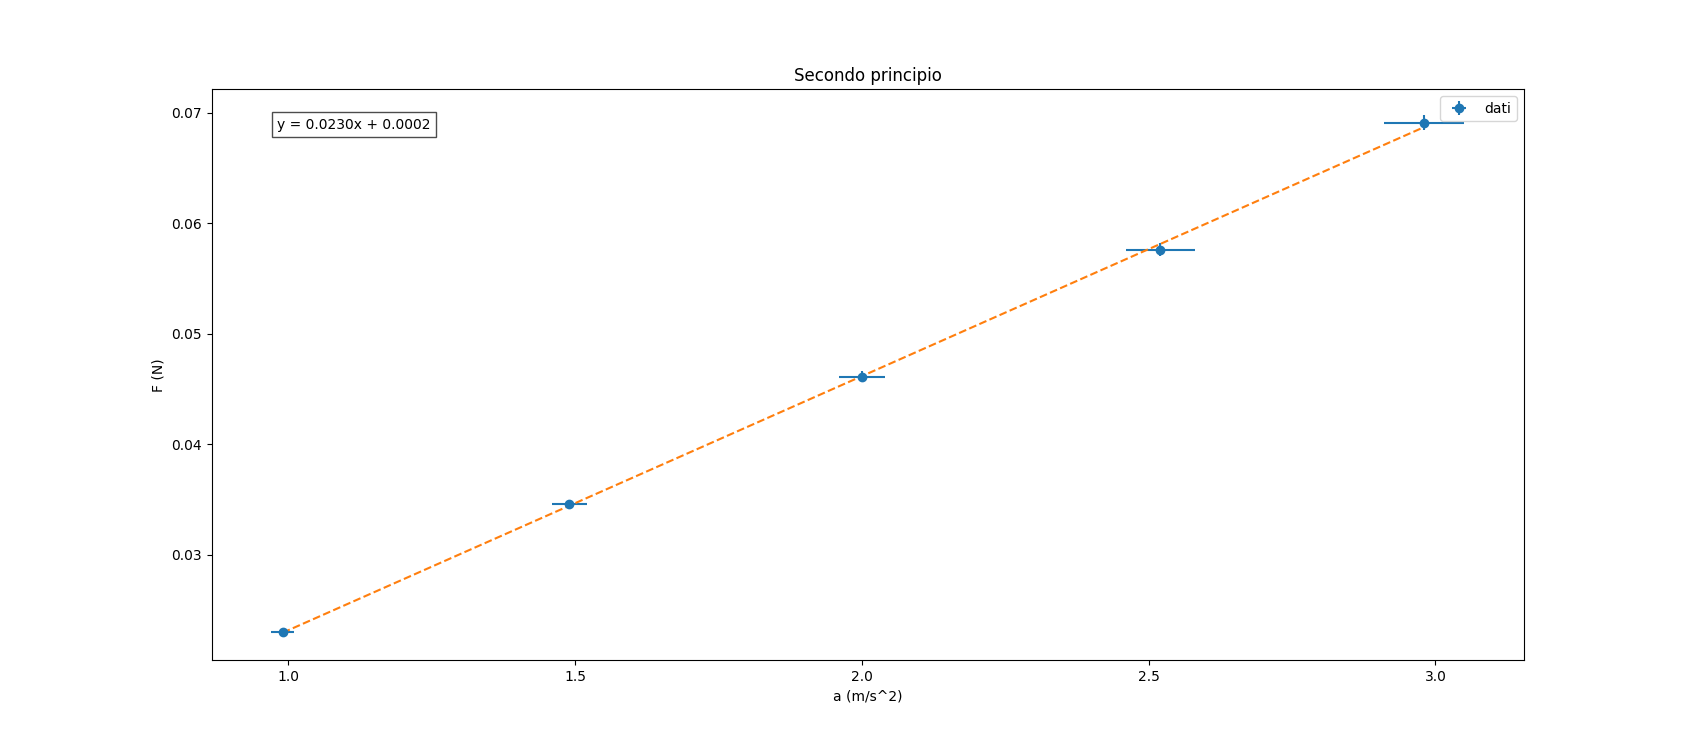
\includegraphics[width=1.2\textwidth]{img/nome_del_file_grafico.png}
\caption{Relazione tra Forza Parallela e Accelerazione}
\label{fig:grafico-pianoinc}
\end{figure}

\subsection{Analisi del Fit Lineare}

Il grafico mostra una chiara relazione lineare tra la forza parallela ($F_\parallel$) e l'accelerazione ($a$). Abbiamo effettuato un fit lineare dei dati, ottenendo la seguente equazione:

\[ F_\parallel = (0,0230 \pm 0,0002) \, \text{kg} \cdot a + (0,0002 \pm 0,0003) \, \text{N} \]

dove $F_\parallel$ è espresso in N e $a$ in m/s$^2$.

\paragraph{Interpretazione dei Risultati:}

\begin{itemize}
    \item \textbf{Pendenza:} La pendenza della retta di best-fit rappresenta la massa dell'oggetto in movimento. Dal fit, otteniamo una massa di $(23,0 \pm 0,2) \, \text{g}$.
    
    \item \textbf{Confronto con la Massa Utilizzata:} La massa reale della pallina utilizzata nell'esperimento era di $23,5 \, \text{g}$. Osserviamo un'eccellente concordanza tra questo valore e quello ottenuto dal fit, con una differenza che rientra ampiamente nell'errore sperimentale.
    
    \item \textbf{Intercetta:} L'intercetta $(0,0002 \pm 0,0003) \, \text{N}$ è compatibile con zero entro l'errore sperimentale, come ci si aspetterebbe da un sistema ideale dove non ci sono forze aggiuntive quando l'accelerazione è nulla.
    
    \item \textbf{Coefficiente di Determinazione:} Il valore di $R^2 = 0,9996$ indica un'eccellente correlazione lineare tra la forza parallela e l'accelerazione, confermando la validità del modello lineare per descrivere la relazione tra queste due grandezze.
\end{itemize}

Questa analisi conferma la validità del nostro esperimento e l'ottima corrispondenza tra i risultati sperimentali e le previsioni teoriche della seconda legge di Newton.

\subsection{Conclusioni}

L'esperimento condotto ha permesso di studiare la relazione tra massa e accelerazione utilizzando un piano inclinato. Dall'analisi dei dati e del fit lineare, emergono le seguenti conclusioni:

\begin{enumerate}
    \item La relazione tra forza parallela e accelerazione mostra una chiara linearità, confermando quantitativamente la seconda legge di Newton ($F = ma$).
    
    \item La pendenza della retta di best-fit, che teoricamente rappresenta la massa dell'oggetto, risulta essere $(23,0 \pm 0,2) \, \text{g}$, in eccellente accordo con la massa reale della pallina $(23,5 \, \text{g})$.
    
    \item La minima discrepanza osservata può essere attribuita a fattori come errori di misura e incertezze strumentali, ma è notevolmente piccola considerando la natura dell'esperimento.
    
    \item L'intercetta prossima a zero conferma l'assenza di forze significative quando l'accelerazione è nulla, in accordo con le aspettative teoriche.
    
    \item L'elevato valore del coefficiente di determinazione (R² = 0,9996) sottolinea l'eccellente correlazione lineare tra le variabili misurate, validando ulteriormente il modello teorico.
\end{enumerate}

Nonostante l'ottima corrispondenza tra i risultati sperimentali e le previsioni teoriche, ci sono sempre margini di miglioramento per future iterazioni dell'esperimento:

\begin{itemize}
    \item Utilizzare strumenti di misura ancora più precisi, specialmente per la misurazione del tempo.
    \item Considerare e quantificare gli effetti dell'attrito nel modello teorico, anche se sembrano essere minimi in questo caso.
    \item Ripetere l'esperimento con diverse masse per verificare la coerenza dei risultati su un range più ampio.
    \item Effettuare una calibrazione ancora più accurata di tutti gli strumenti prima dell'esperimento.
\end{itemize}

In conclusione, l'esperimento ha confermato con notevole precisione la relazione lineare tra forza e accelerazione prevista dalla seconda legge di Newton. La qualità dei risultati ottenuti testimonia l'accuratezza delle misurazioni e l'efficacia del setup sperimentale utilizzato.


